\section{Etudes préalables}

Avant de commencer à parler de tout l’aspect technique et conception nous allons resituer notre projet en définissant ses objectifs, son plan de route et ses inspirations.

\subsection{Présentation du projet}

Ce projet a été mis en place de notre propre initiative et nous avons donc défini les objectifs à atteindre ainsi que les fonctionnalités de nous-même, avec l'aide du tuteur de projet.

L’idée originelle que nous avions proposée était inspirée de la carte du Maraudeur de l’univers Harry Potter visible sur la figure \ref{marauder}. Cette carte permet grâce à la magie de suivre en temps réel toutes les personnes présentes à Poudlard, l’école de sorciers, puisque leurs pas apparaissent dessus avec leur nom. Cet objet, bien que magique, nous semblait aujourd’hui pouvoir être réalisé grâce aux avancées liées au domaine des objets connectés. 

\begin{figure}[H]
    \centering
    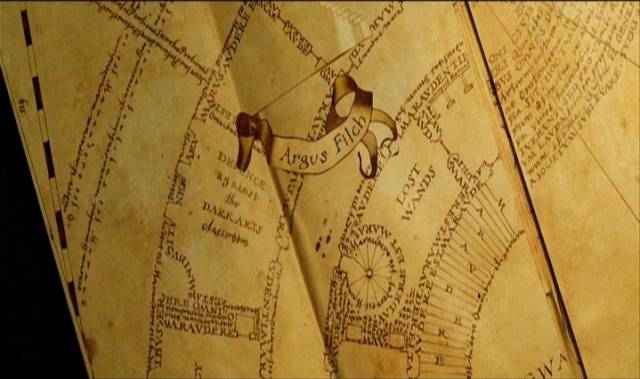
\includegraphics[width=\textwidth]{./img/marauder.jpg}
    \caption{Morceau de la carte du Maraudeur tirée du film Harry Potter}
    \label{marauder}
\end{figure}

Nous avons donc décidé de proposer une manière simple pour tout le monde de pouvoir s'orienter et retrouver des personnes dans les locaux de l'ISIMA au travers d’une application. Cette solution devra donc récolter un ensemble des données sur les usagers de l’ISIMA et les reporter sur une carte qui sera bien sûr électronique. Nous voulons ainsi que chacun puisse sortir notre carte de sa poche pour retrouver un ami ou un collègue instantanément.

De manière générale, nous devons être capable de visualiser une carte de l'ISIMA, mais également de pouvoir trouver facilement une personne, un bureau ou une salle de cours. De plus, il serait intéressant de pouvoir faire ceci en temps réel. L'actualisation des données doit donc être assez rapide pour que la localisation des utilisateurs soit la plus précise possible.

Une fois cette solution éprouvée avec les bâtiments de l'ISIMA, nous pouvons penser l'étendre à n'importe quel autre bâtiment dont nous pouvons avoir les plans. L’intérêt ici étant de développer une preuve de fonctionnement du suivi de personnes dans un bâtiment qui plus est considéré comme étant très surchargé de signaux. Comme nous l’évoquions plus tôt ceci pourrait trouver différentes utilisations dans différents contextes comme par exemple le fonctionnement d’un hôpital, la surveillance d’une prison, l’évacuation d’un bâtiment. Avec l’avènement de l’open data, il y a aussi de nombreuses questions éthiques à résoudre vis-à-vis des informations récoltées et diffusées. La CNIL au travers de la loi Informatique et Libertés règlemente l'utilisation de la géolocalisation d'employés dans une entreprise \cite{loigeo} en mettant en avant les droits des employés : il faut que cette géolocalisation est une finalité claire et prédéterminée, que les données ne soient pas conservées plus longtemps que prévu, l'employé doit avoir connaissance du dispositif et doit pouvoir l'interrompre. Toutefois, la CNIL n'est pas très précise quant à la géolocalisation de particuliers. Il existe aussi une directive européenne sur les traceurs \cite{cookies} qui demande à ce que les internautes donnent leur consentement avant l'introduction d'un traceur, par exemple un cookie. Cette demande de consentement existe déjà plus ou moins sur les applications Android puisque lors de l'installation d'une application, celle-ci fait part du besoin d'accéder au gps, ce que l'utilisateur est libre d'autoriser ou non. A ceci on peut rajouter les lois sur la protection de la vie privée et des données personnelles.

Il faut aussi se demander comment notre application va se positionner par rapport aux applications existantes. Pour ce faire nous allons maintenant aborder l’analyse de l’existant.


\subsection{Analyse de l'existant}

Nous ne nous attarderons pas dans cette partie sur la carte magique imaginée par J. K. Rowling mais nous allons plutôt voir les différentes applications existant autour de la localisation d’usagers.

Le premier exemple est celui des réseaux sociaux. En effet, avec leur avènement est arrivé aussi un moyen pour des grands groupes de récolter une masse importante d’information sur leurs utilisateurs : ce que l’on appelle le Big Data. Dans cette masse de données, il y a bien évidemment des données de géolocalisation. Celles-ci sont de plusieurs types : soit données, soit mesurées.

Les premières, dites données, sont les informations que l’utilisateur va donner de lui-même aux réseaux sociaux comme par exemple poster une photo d’une après-midi entre amis en spécifiant le lieu de la prise de vue. Cette information peut être légitimement utilisée puisque donnée par l’utilisateur mais cela ne représente pas une source fiable ni même précise. Même si cette information n’est pas fiable, les réseaux sociaux ont trouvé depuis 2014 une toute nouvelle utilisation à ce type d’information : l’aide aux personnes en danger. En effet, Facebook a développé un service nommé Safety Check \cite{fbsafetycheck} qui repère les personnes présentes à proximité d’une zone de danger que ce soit une catastrophe naturelle ou bien encore une action terroriste et leur propose de se signaler en sécurité auprès de leurs proches. Le Safety Check visible à la figure \ref{safety-check} est un bon exemple de localisation de personnes mais demande à ce que les personnes recherchées effectuent une action.

\begin{figure}[H]
    \centering
    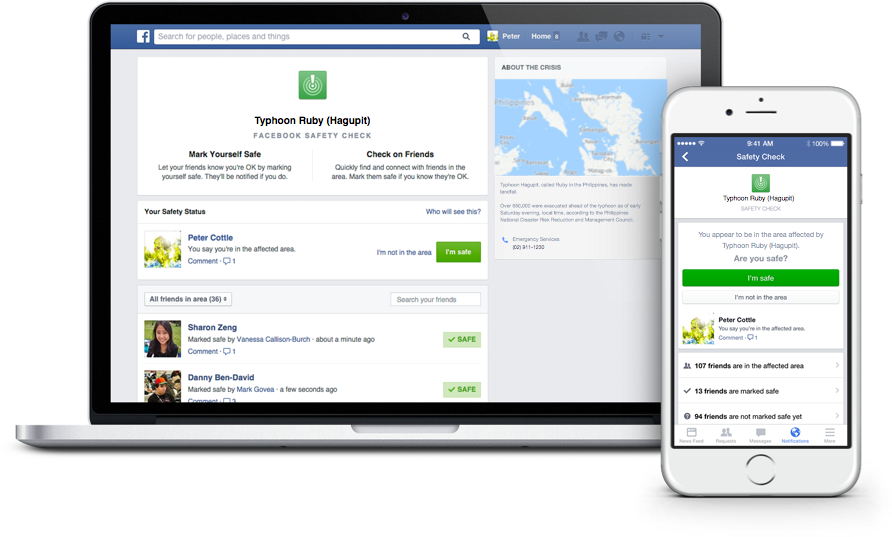
\includegraphics[width=\textwidth]{./img/safetycheck.png}
    \caption{Service Safety Check de Facebook}
    \label{safety-check}
\end{figure}

Le second type dit données mesurées représente toutes les informations que les réseaux sociaux récupèrent sur les appareils des utilisateurs. Cette récupération est rendue possible tout d’abord par l’existence de ces données. En effet depuis quelques années avec l’arrivée des smartphones et des objets connectés, la majeure partie des appareils électroniques possèdent des fonctionnalités de géolocalisation. Il est alors facile pour une application d’accéder à la position de son utilisateur. En général, l’appareil en question est un smartphone et se trouve très souvent au même endroit que son propriétaire, voire sur lui-même. On peut clairement constater la récupération de ces informations lorsque la localisation d’un utilisateur est associée directement au message qu’il poste ou bien encore sur les historiques. En effet, Google propose à ses utilisateurs d’accéder à tout l’historique de leurs déplacements \cite{bibgoogle} comme on peut le voir sur la figure \ref{google-maps}. Google récupère en permanence la position de utilisateurs afin de pouvoir fournir à la communauté des statistiques sur l’affluence de certains lieux, de demander des informations et photos sur les lieux en cours de visite ou bien proposer des services à proximité. Google arrive ici à localiser avec précision dans quel établissement une personne se trouve mais ne partage pas les données individuelles au reste de la communauté.

\begin{figure}[H]
    \centering
    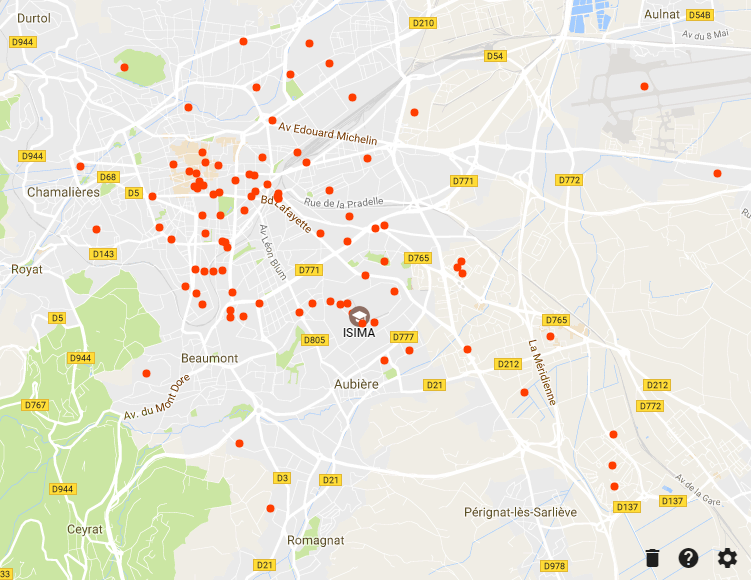
\includegraphics[width=\textwidth]{./img/googlemaps.png}
    \caption{Suivi des déplacements sur Google Maps}
    \label{google-maps}
\end{figure}

Les réseaux sociaux sont donc un acteur de premier plan dans la géolocalisation de personnes puisqu’ils disposent de nombreuses données sur le sujet mais ne diffusent qu’une fraction de celles-ci. Nous allons maintenant voir qu’il existe des services plus ouverts.

\subsubsection{Les services open data}

Dans les communautés de développeurs le phénomène open source qui consiste à partager librement les sources de ses propres programmes connaît beaucoup de succès. Sur cette base a émergé un nouveau concept : celui de l’open data. Comme son nom l’indique l’open data consiste à partager des données utiles récoltées.

Ces données sont le plus souvent fournies sous la forme d’un service web ou bien d’un fichier facilement découpable et analysable comme un fichier xml ou csv. L’intérêt est que ces données soient réutiliser par d’autres personnes en vue de concevoir un service plus consistant que des données brutes. Ainsi on donne aux développeur le moyen de concevoir des applications se basant sur de vraies données ce qui a pour effet de motiver l’innovation et la concurrence dans un domaine.

Un des exemples les plus connus en France et qui rejoint notre projet est celui de la société Keolis qui gère le service de transport en commun de la ville de Rennes. Cette société a décidé depuis sept ans déjà d’offrir au grand public des données utiles sur son activité de transport dans la ville de Rennes. En outre, Keolis a équipé ses bus de balises gps et partage en temps réel la position des bus des différentes lignes \cite{stardataexplore}. Il y a deux avantages à cette ouverture pour Keolis : la communauté des développeurs peut concevoir d’innombrables applications reposant sur des données sans cesse renouvelées et ainsi disposer sans efforts des meilleurs services mobiles en matière de transport en France. En effet, en comparaison d’une ville comme Clermont-Ferrand où les applications de transports reposent sur les horaires fixes décidés en début d’année, la ville de Rennes propose une application souple qui s’adapte même aux retards individuels de chaque véhicule.

Comme on peut le voir sur la figure \ref{rennes}, la flotte rennaise peut être localisée à tout instant.

\begin{figure}[H]
    \centering
    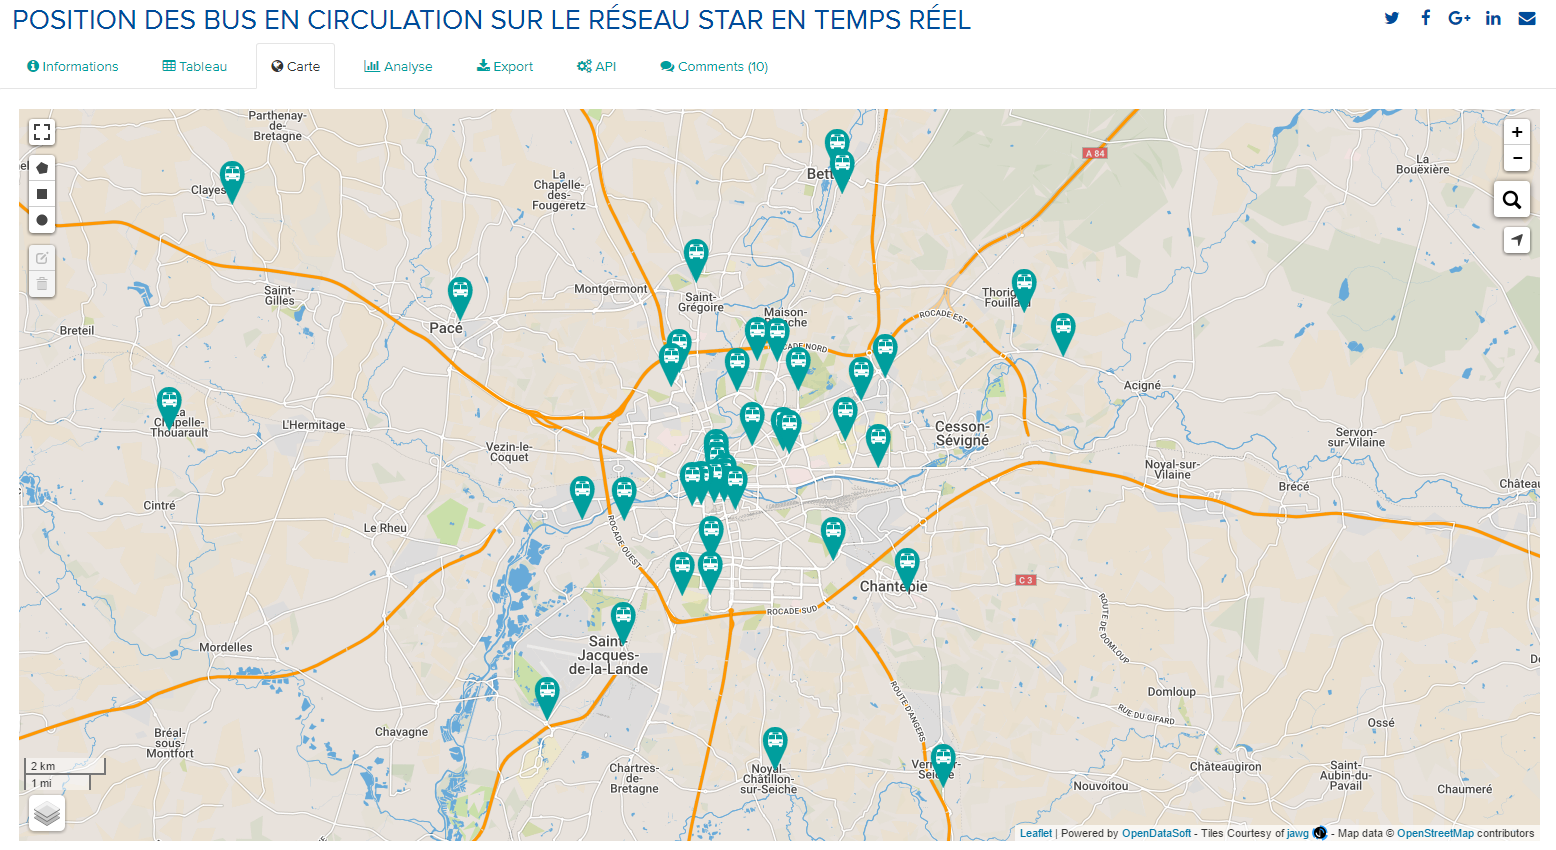
\includegraphics[width=\textwidth]{./img/rennes.png}
    \caption{Localisation en temps réel des bus de la ville de Rennes}
    \label{rennes}
\end{figure}

Dans ce cas, il est vrai que l’on ne parle pas de localiser directement des personnes mais des véhicules. Cependant des problèmes similaires se posent et se sont posés à commencer par la protection de l’identité. En effet, le service web proposait initialement d’obtenir pour chaque bus son numéro d’identification mais ceci permettait de suivre un véhicule en permanence. On peut imaginer beaucoup de choses sur l’utilisation d’une telle information. A chaque véhicule étant associé un chauffeur, n'importe qui pouvait donc localiser un chauffeur en temps réel dans le cadre de l'exercice de ses fonctions mais cette fonctionnalité a été retirée puisqu’elle n’apportait rien de plus aux usagers.

Il y a donc possibilité de produire des applications qui donnent accès à des positions en temps réel au grand public mais celles-ci posent vite des problèmes d’éthique et légaux. Nous allons donc voir les applications réelles qui existent sur la localisation de personnes.

\subsubsection{Les applications similaires}

Dans la plupart des recherches effectuées, on trouve des dispositifs électroniques permettant de suivre une personne dépendante comme un enfant, une personne âgée ou handicapée.

Par exemple la société Geotek propose à ses clients des boitiers GSM permettant de localiser une personne \cite{bibgeotek}. Ils proposent leur utilisation pour les personnes dépendantes et même pour l’optimisation des déplacements d’employés dans une entreprise. Cette offre se rapproche un peu plus de notre projet mais s’en éloigne un peu dans le sens où elle nécessite l’utilisation de matériel supplémentaire et concerne la localisation de seulement quelques personnes auprès d’une seule personne.

En cherchant sur le Google Play qui est la plateforme officielle de téléchargement des applications Android on trouve quelques applications de localisation. Ces applications prennent bien souvent la forme de réseaux sociaux pour les soucis de confidentialité évoqués plus tôt.

Dans cette catégorie on peut parler de Find My Friends \cite{bibfindmyfriends} produite par Family Safety Production (figure \ref{findmyfriends}). Cette application propose des fonctionnalités intéressantes puisqu’elle permet de localiser ses amis qui possèdent l’application. Mais ce n’est pas tout, ils proposent aussi de pouvoir localiser les personnes qui n’ont pas l’application en envoyant juste un SMS à cette personne et si elle répond « oui » sa position s’affiche chez le demandeur. Cette fonctionnalité est très intéressante car elle permet de s’abstraire de l’application chez une partie des personnes.

\begin{figure}[H]
    \centering
    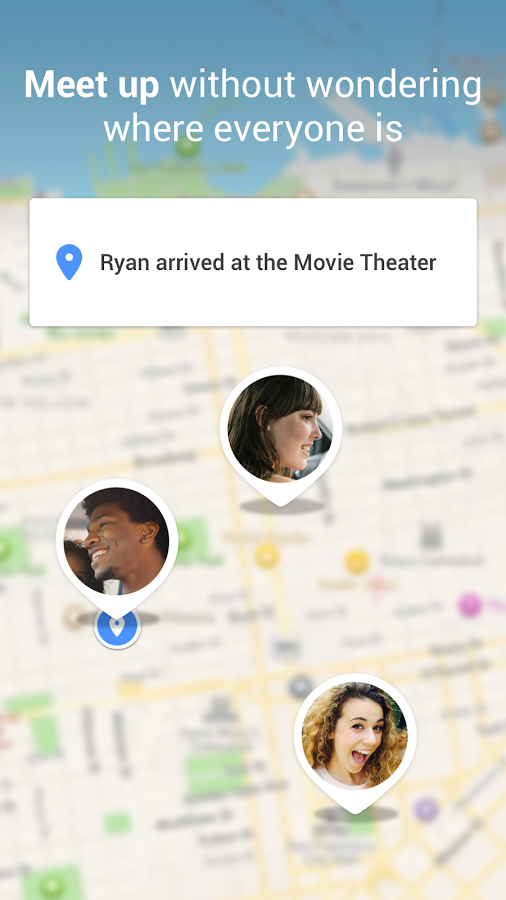
\includegraphics[height=8cm]{./img/findmyfriends.png}
    \caption{Application Find My Friends de Family Safety Production}
    \label{findmyfriends}
\end{figure}

Dans le même estprit on retrouve aussi l'application Foursquare. Cette application permet aux utilisateurs de se géolocaliser auprès des autres dans lieux comme des magasins. A ceci est associé un système de gamification, c'est-à-dire que des passages répétés dans un même endroit permet de gagner des badges en récompense. Foursquare proposait aussi de trouver le domicile des utilisateurs et les contacts à proximité. La fonctionnalité signalement du domicile a cependant été modifiée par soucis de confidentialité.

Le point étant fait sur les applications existant nous allons maintenant définir plus précisément ce que nous souhaitons proposer au travers de notre application.


\subsection{Spécifications du projet}

Etant donné que peu de solutions sont disponibles sur le marché, nous avons choisi de partir de zéro et créer notre solution. Cela nous permet également d'avoir un contrôle total sur les données du projet, les diverses implémentations de fonctionnalités ainsi que la manière dont nous souhaitons utiliser notre solution.

La solution la plus évidente en termes de support de visualisation pour les utilisateurs est de leur proposer une application qu'ils pourront installer sur leur smartphone, PC, montre connectée ou encore tablette.

Afin de rendre cette application dynamique et de proposer un suivi de position d'utilisateurs en temps réel, il est convenu d'utiliser un service web. Ce service devra également pouvoir stocker des informations utiles aux utilisateurs, ce qui permettra également d'alléger le volume de données stockées sur leurs terminaux.

Nous allons donc détailler dans la suite les principaux éléments que nous voulons produire pour donner une vision de l’objectif final que nous souhaitons atteindre.

\subsubsection{Architecture}

Tout d’abord nous souhaitons fournir un service à un groupe de personnes plutôt important : nous avons donc besoin d’une architecture qui puisse gérer plusieurs utilisateurs sur une même application. L'architecture choisie pour organiser notre solution en est une de type client-serveur comme elle peut être décrite sur la figure \ref{architecture}.

\begin{figure}[H]
    \centering
    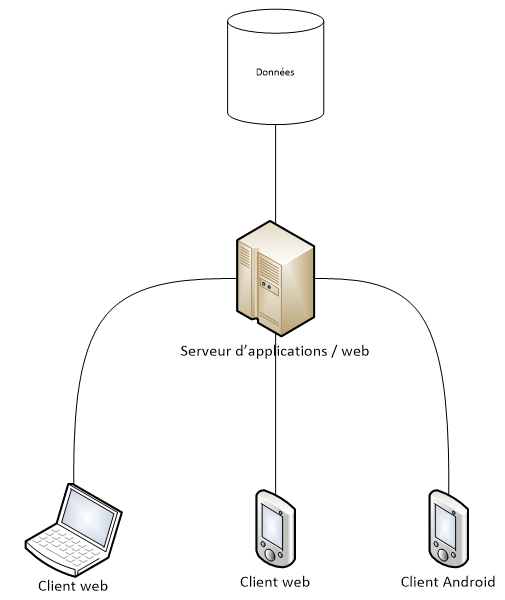
\includegraphics[height=10cm]{../infrastructure.png}
    \caption{Architecture générale de la solution}
    \label{architecture}
\end{figure}

Nous pouvons donc observer sur cette figure un schéma tout à fait classique de système client-serveur qui nous permettra de dissocier le développement du service du développement des différentes interfaces utilisateur. Un intérêt majeur est de pouvoir faire évoluer un des clients sans que cela n’impacte le cours de vie des autres projets reposant sur le service ou le service lui-même.

Pour ce faire nous allons donc développer un service web de type REST~\cite{rest} pour que différents clients, illustrés dans notre projet par un client Android, puissent l’utiliser avec un minimum de contraintes. Les évolutions du serveur et du client n’auront donc pas d’impact l’un sur l’autre sauf bien sûr sur les modifications de l’interface. Si jamais un problème se déclarait dans la conception d’une partie nous comptons sur notre système d’intégration continue pour jouer le rôle de garde-fou en contrôlant le code versionné.

Nous allons maintenant aborder en détails les objectifs fixés pour chacun de ces éléments.

\subsubsection{Partie serveur}

Le serveur est le point reliant tous les clients et possèdent différents services mais la partie centrale est celle du service web. Le serveur doit être capable de répondre aux différentes connexions et requêtes des utilisateurs se connectant depuis l'application Android ou depuis tout autre client. Un service web n’est autre qu’un ensemble de services distants disponibles sur internet, ils peuvent permettre de récupérer des données ou bien d’effectuer des traitements spécifiques. L’intérêt est que le mode de communication avec un service web se veut standard ce qui permet à des utilisateurs de topologie différentes de le consommer.

Le serveur sera un service web de type \textbf{REST} c’est-à-dire qu’il sera capable de répondre à des requêtes http dans un format standardisé, le \underline{JSON}. Ce type de service est de plus en plus répandu car il est supposé \textbf{sans état} du client sur le serveur, effectue des requêtes \textbf{auto-descriptives} (informations sur son contenu, sa date de création, son expiration, ...) sur des \underline{URL} \textbf{identifiant} des ressources de manière \textbf{précise}. Ceci en fait donc une base idéale pour les architectures basées sur des services web.

Le serveur disposera des fonctionnalités minimales suivantes :

\begin{itemize}
    \item un système d’authentification afin de valider l’identité des utilisateurs ;
    \item un service de collection des positions des utilisateurs ;
    \item un service d’obtention de la liste des personnes connectées ;
    \item un service de récupération de la position actuelle de l'utilisateur connecté ;
    \item un système de connexion/déconnexion des utilisateurs.
\end{itemize}

Ces fonctionnalités seront essentielles pour le fonctionnement de base de l'ensemble de la solution. Par la suite, des fonctionnalités supplémentaires pourront être ajoutées dans l'application, comme par exemple :

\begin{itemize}
    \item un historique des positions ;
    \item un service de calcul d'itinéraire entre deux positions dans le bâtiment ;
    \item un service de partage de position (par sms, mail, etc.).
\end{itemize}

Pour stocker les diverses informations utilisateur (login, position), nous avons convenu d'utiliser une base de données qui s'interfacera directement avec le service web.

L’ensemble devra donc être disponible sur une machine atteignable sur internet et devra avoir une haute disponibilité. C’est pourquoi il n’est pas concevable de le déployer sur un ordinateur personnel. Deux solutions s’offrent donc à nous :

\begin{itemize}
    \item l’utilisation d’une machine dédiée autogérée ;
    \item la location d’un IaaS ou CaaS (Infrastructure/Container as a Service).
\end{itemize}

La première solution consiste à utiliser une machine personnelle connectée en permanence à internet depuis notre domicile et la seconde à louer un service chez un fournisseur comme Amazon ou Google qui pourrait soit être une machine virtuelle Linux soit un conteneur d’applications. Le format aaS est à privilégier pour des raisons de performances et de disponibilité mais nous verrons que des soucis de budget nous ont conduit à opter pour la première solution.

Nous avons fait le tour de ce à quoi devra ressembler le serveur, abordons maintenant la question du client.

\subsubsection{Partie Android}

La seconde partie de ce projet concerne le client qui sera une application Android mais qui pourrait tout aussi bien être déclinée pour iOS et Windows Universel. Cette application sera donc une interface entre l’utilisateur et le service et devra lui permettre de profiter des fonctionnalités minimales attendues par rapport à la carte du maraudeur de Harry Potter.

Les fonctionnalités majeures seront donc :
\begin{itemize}
    \item l’inscription ;
    \item la connexion-déconnexion ;
    \item l’envoi de sa position gps au service web ;
    \item la réception des positions gps d'autres utilisateurs connectés ;
    \item la visualisation en temps réel sur une carte des positions.
\end{itemize}

Ces fonctionnalités forment le noyau dur indispensable au niveau minimal de qualité de notre application. Des améliorations sont envisageables pour augmenter le niveau de service, ainsi l'application pourra évoluer et proposer :
\begin{itemize}
    \item une carte en version 3D ;
    \item une carte en version réalité virtuelle ;
    \item le partage de position ;
    \item l'ajout d'informations sur la carte (lieu / point de rdv).
\end{itemize}

La mise à jour des informations sur le client sera initiée par l’application qui effectuera une requête sur le serveur. Le serveur renverra les positions des utilisateurs connectés qui permet sa mise à jour chez les utilisateurs.

Le choix d'une application Android se justifie par plusieurs facteurs. Tout d’abord il existe une communauté très active et de nombreux documents autour de l’Android. Ceci est dû en grande partie que le marché est majoritairement composé de terminaux Android, il y a donc plus de références et de documentation. Enfin le langage Android se basant sur du Java il nous est plus accessible de partir sur cette plateforme plutôt que sur du iOS ou même du Windows Universel, de plus nous avons quelques notions en Android.

Les versions du framework Android qui seront supportées seront les version 11 et ultérieures pour fonctionner sur un maximum de terminaux. Toutefois la version de compilation sera la 25 afin de pouvoir profiter des dernières mises à jour du framework. Ceci est rendu possible grâce aux ressources de post-compatibilité Android (appcompat) qui apportent aux terminaux plus anciens certaines des améliorations non-existantes dans leur version.

Nous aurions pu faire le choix de développer dans une technologie cross-plateform se basant sur des technologies web comme Ionic mais nos besoins en accès matériel de part le gps et \underline{OpenGL} nous semblait être en désaccord avec un tel choix.

Nous allons maintenant aborder un aspect important dans le développement de ce projet : son intégration continue.

\subsubsection{Intégration continue}

Un des objectifs de ce projet est de mettre en place une intégration continue et un déploiement automatique.

Dans les milieux industriels, le développement de solutions comporte souvent 3 phases :
\begin{itemize}
    \item L'analyse ;
    \item Le développement ;
    \item Les tests et l'intégration.
\end{itemize}

Cette dernière étape est l'une des plus importantes, puisque c'est au cours de cette phase que la solution va être validée à l'aide de tests de non-régréssion, puis mise en production afin d'être livrée à ses clients. C'est ce que l'on appelle la phase d'intégration continue, qui permet d'assurer la qualité du code tout au long de l'évolution de la solution.

Cette phase est généralement automatisée afin de libérer du temps aux développeurs, éviter des tâches répétitives, mais surtout permettre l'élimination d'erreurs humaines et assurer la reproductibilité des builds et des tests. Ces dernier critères sont assurés par la présence de fichiers de configuration de l'intégration continue qui sont versionnés au même titre que le code la solution. Ainsi, ces fichiers évoluent en même temps que la solution elle-même.
Des outils sont donc disponibles sur le marché pour effectuer ces tests de non-régréssion et effectuer l'opération menant à l'établissement d'une version de production pour la solution visée.

Nous avons donc vu à quoi notre solution vise à ressembler, nous allons maintenant développer notre stratégie de planification du travail.

\subsection{Organisation du travail}

L'organisation temporelle théorique du travail est décrite dans le diagramme de Gantt de la figure \ref{ganttinit}. Elle se veut assez simple et découpée en quatre phases :

\begin{itemize}
    \item la phase de lancement qui s’étend jusqu’à la rentrée des vacances de la Toussaint et comporte toutes les travaux d’analyse et de mise en place du projet ;
    \item la phase de développement basique qui s’étend jusqu’à début 2017 et concerne le développement des applications minimales du projet.
    \item la phase d’amélioration durant laquelle l’ajout d’améliorations supplémentaires sera fait à l’application de base ;
    \item la phase de finalisation comportant la préparation de la documentation autour du projet.
\end{itemize}

La première phase est celle qui se prête le plus à un travail commun, puis les phases suivantes ont été pensé de façon modulaire afin de pouvoir travailler indépendamment de l’autre sur chaque tâche. Nous verrons plus tard comment le déroulement du projet a eu lieu dans les faits et quelles modifications de planning ont été apportées.

Nous avons discuté des différents points caractérisant notre projet et les objectifs que nous souhaitions atteindre, nous allons maintenant expliquer comment nous nous y sommes pris pour la conception dans la section suivante.

\begin{landscape}
    \begin{figure}[h]
        \centering
        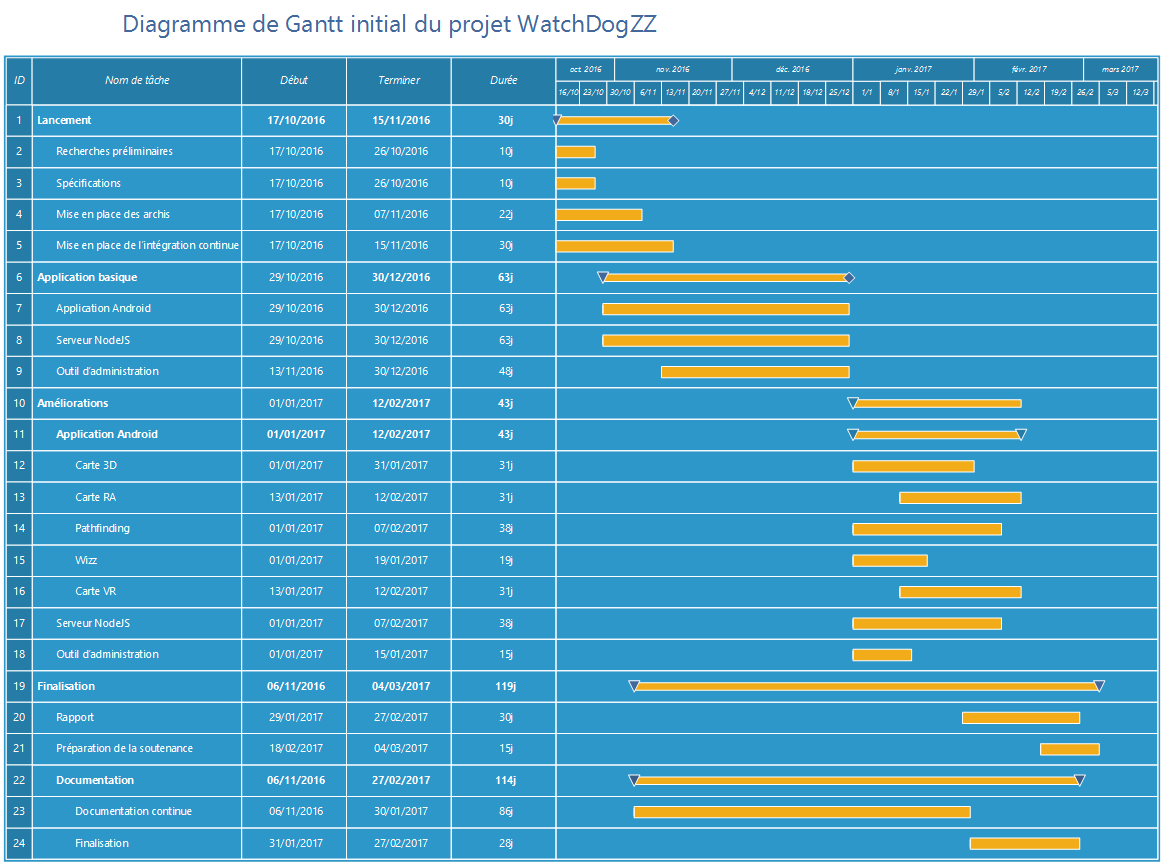
\includegraphics[height=\textwidth]{../gantt_initial.png}
        \caption{Diagramme de Gantt théorique}
        \label{ganttinit}
    \end{figure}
\end{landscape}
